\subsection{Хэш-функции}
Хэш-функция –- это математическая функция, принимающая на вход данные произвольного размера и преобразующая их в выходные данные фиксированного размера.

Сфера применения хэш-функций в криптографии включает аппарат для проверки целостности пересылаемого сообщения (аутентификация сообщения), идентификации пользователя по паролю, вычисления электронной цифровой подписи (обеспечения невозможность отказа от авторства) и др. 
Хэш-функции, применимые в области криптографии, называются криптографическими хэш-функциями.

Дадим определение криптографической хэш-функции. 

 \textbf{Определение.} Криптографическая хэш-функция -- это отображение $H\colon V^* \rightarrow V_n$, где $n\in \mathbb{N}, \ V^*$ -- множество всех двоичных векторов конечной размерности, включая пустую строку, $\ V_n$ -- множество всех n-мерных двоичных векторов. Хэш-кодом будем называть результат применения к сообщению $m$ хэш-функции $H = H(m)$.

Криптографическая хэш-функция должна соответствовать следующим критериям \cite{criteria}:
\begin{enumerate} 
\item Стойкость к поиску прообраза (по заданному значению хэш-функции $H(m)$ сложно найти значение сообщения $m$);
\item Стойкость к поиску второго прообраза (по заданному сообщению $m_1$ сложно вычислить сообщение $m_2$, для которого $H(m_1) = H(m_2)$ при $m_1 \neq m_2$);
\item Стойкость к коллизиям (сложно вычислить значения сообщений $m_1 \neq m_2$, для которых $H(m_1) = H(m_2)$).
\end{enumerate}

\subsubsection{Задачи криптографических хэш-функций}
Задачи, которые рассматриваются при анализе криптографических хэш-функций, следуют из критериев, описанных выше. 

\begin{enumerate} 
\item Аутентификация сообщений \\
Аутентификация сообщения – это процедура установления подлинности предъявляемого идентификатора взаимодействия (например, проверка, что содержание сообщения не было изменено во время пересылки от отправителя к получателю). В зависимости от возможностей злоумышленника задача нарушения целостности сводится к задачам построения первого и второго прообразов и коллизии используемой хэш-функции.
\item Идентификация пользователя по паролю \\
Зачастую для проверки правильности введенного пароля происходит не его сравнение с (эталонным) паролем, а вычисление хэш-кода от этого пароля и последующее сравнение с хэш-кодом, хранящимся в базе данных \cite{hash_password}. В этом случае для того, чтобы подделать пароль и получить несанкционированный доступ к ресурсу, необходимо решить задачу построения прообраза функции хэширования. 
\item Невозможность отказа от авторства \\
Для обеспечения невозможности отказа от авторства используется механизм вычисления электронной цифровой подписи (ЭЦП). Криптографическая стойкость ЭЦП зависит от трудоемкости решения задач построения первого и второго прообразов и коллизии хэш-функции.
\end{enumerate}

\textbf{Методы анализа хэш-функций:}
\begin{enumerate} 
\item Метод тотального перебора сообщений  
\item Метод поиска коллизий на основе атаки «дней рождения» \cite{birthday_attack}
\item Метод параллельного поиска коллизий \cite{parallel_col}
\end{enumerate}

Одним из направлений криптографии, в котором используются хэш-функции, является вычисление электронной цифровой подписи. Алгоритм вычисления подписи относится к асимметричной криптографии с открытым ключом. Отправитель создает пару ключей: секретный ключ и открытый ключ. Пользователь хранит секретный ключ в тайне и может использовать его для создания цифровой подписи для любого сообщения. Только пользователь-владелец секретного ключа может подписать сообщение от своего имени при условии, что он надежно хранит эту часть ключа. 

Алгоритм подписи в качестве входных данных принимает сообщение и секретный ключ. После подписания сообщения, он добавляет полученную подпись $s$ к сообщению $m$ и отправляет пару $(s,\ m)$ получателю.

Первым идею использования хэш-функций для создания цифровых подписей (One-Time Signature) озвучил Лесли Лэмпорт в 1979 году \cite{lamport}.

\begin{figure}[h]
\centering
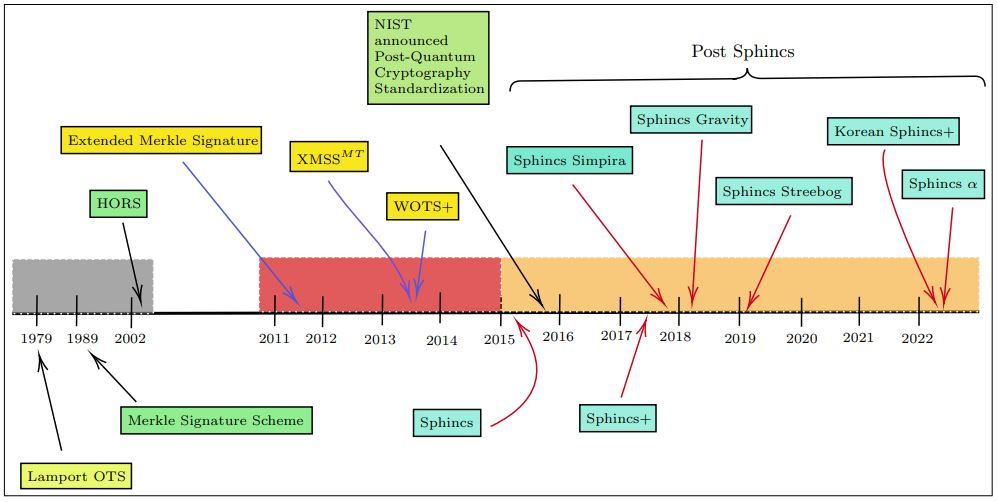
\includegraphics[scale=0.6]{images/timeline.jpg}
\caption{Хронология развития алгоритмов ЭЦП на основе хэш-функций \cite{timeline}}
\end{figure}

\subsubsection{SPHINCS$^+$}

SPHINCS$^+$ -- это алгоритм ЭЦП на основе хэш-функции, выбранный в качестве финалиста второго раунда конкурса стандартизации алгоритмов постквантовой криптографии от NIST. 

 Введем несколько понятий, используемых в аппарате алгоритма SPHINCS+.

\textbf{Определение.} Гипердерево -- это дерево многоразовых подписей на основе хэш-функции.

\textbf{Определение.} Хэш-дерево -- это полное двоичное дерево, в листовые вершины которого помещены хэши от блоков данных, внутренние вершины содержат хэши от сложения значений в дочерних вершинах, а корневой узел дерева содержит хэш от всего набора данных.


Схема SPHINCS+ использует гипердерево Меркла, состоящее из множества бинарных хэш-деревьев, которые соединены между собой одноразовой схемой подписи (Winternitz-type OTS) WOTS$^+$. Открытый ключ хранится в корне гипердерева. В нижней части гипердерева используется малократная подпись (Forest of Random Subsets) FORS.

Например, гипердерево схемы подписи SPHINCS$^+$ можно изобразить следующим образом:

\begin{figure}[H]
\centering
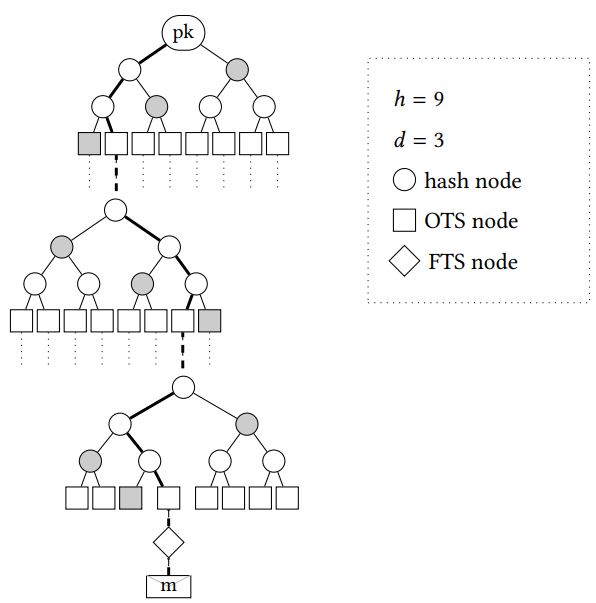
\includegraphics[scale=0.8]{images/sphincs+.JPG}
\caption{Cхема алгоритма SPHINCS$^+$ \cite{sphincs_scheme}}
\end{figure}

\textbf{Достоинства и недостатки алгоритма SPHINCS$^+$ }\cite{doc_sphincs}

Недостаток: размер подписи и скорость.

Достоинства: 
\begin{itemize}
\item 
безопасность SPHINCS$^+$ основана на
предположениях о безопасности используемой хэш-функции;
\item
наиболее эффективные известные атаки против SPHINCS$^+$ легко установить и проанализировать;
\item
небольшой размер ключей, в частности размер открытого ключа (несомненное преимущество при частой передаче сертификатов, например, SSL/TLS).
\end{itemize}